\documentclass{article}

% -------------------------------------
%           PACKAGES
% -------------------------------------
\usepackage[french]{babel}
\usepackage[T1]{fontenc}
\usepackage[utf8]{inputenc}
\usepackage[a4paper, top=2cm, bottom=2cm, left=2.5cm, right=2.5cm]{geometry}
\usepackage{graphicx}
\usepackage{xcolor}
\usepackage{tikz}
\usepackage{fancyhdr}
\usepackage[hidelinks]{hyperref}
\usepackage{titlesec}
\usepackage{framed}
\usepackage{amsmath}
% -------------------------------------
%     COULEURS FIND & ORDER
% -------------------------------------
\definecolor{foblue}{HTML}{27C7D8}
\definecolor{foorange}{HTML}{F05A2A}
\definecolor{foyellow}{HTML}{F8C43E}
\definecolor{lightgray}{gray}{0.95}

% -------------------------------------
%         TITRES COLORÉS
% -------------------------------------
\titleformat{\section}
  {\Large\bfseries\color{foorange}}
  {\thesection}{1em}{}

\titleformat{\subsection}
  {\large\bfseries\color{foblue}}
  {\thesubsection}{1em}{}

% -------------------------------------
%        CADRE THÉMATIQUE
% -------------------------------------
\newenvironment{thematique}{
\def\FrameCommand{\colorbox{lightgray}}
\MakeFramed{\advance\hsize-\width \FrameRestore}
}{
\endMakeFramed
}

% -------------------------------------
%     ENTÊTES & PIEDS DE PAGE
% -------------------------------------
\pagestyle{fancy}
\fancyhf{}
\lhead{
\includegraphics[width=1.6cm]{images/logo.jpeg}}
\rhead{\textcolor{foblue}{}}
\cfoot{\thepage}
\renewcommand{\headrulewidth}{0pt}

% -------------------------------------
%     PAGE DE GARDE PERSONNALISÉE
% -------------------------------------
\newcommand{\pagedegarde}{
\begin{titlepage}
    \centering

    % Barre tricolore supérieure
    \begin{tikzpicture}[remember picture, overlay]
        \fill[foblue] (0,0) rectangle (2,0.26);
        \fill[foorange] (2,0) rectangle (3.5,0.26);
        \fill[foyellow] (3.5,0) rectangle (5,0.26);
    \end{tikzpicture}

    \vspace*{2cm}

    % Zone logos
    \begin{minipage}{0.45\textwidth}
        \centering
        
\includegraphics[width=0.75\textwidth]{images/logo.jpeg}
    \end{minipage}
    \hfill
    \begin{minipage}{0.45\textwidth}
        \raggedleft
        
\includegraphics[width=0.80\textwidth]{images/logo_bdx.png}
    \end{minipage}

    \vspace{3cm}

    % TITRE
    {\Huge \bfseries Projet professionnel 2026}\\[0.8cm]
    {\Large Optimisation des flux de préparation en entrepôt}\\[2cm]

    {\large Find \& Order \\ Janvier 2026}

    \vfill

    % Barre tricolore inférieure (identique à celle du haut)
    \begin{tikzpicture}[remember picture, overlay]
        \fill[foblue] (0,0.3) rectangle (2,0.55);
        \fill[foorange] (2,0.3) rectangle (3.5,0.55);
        \fill[foyellow] (3.5,0.3) rectangle (5,0.55);
    \end{tikzpicture}

\end{titlepage}
}

% -------------------------------------
%         DOCUMENT
% -------------------------------------
\begin{document}

\pagedegarde

\tableofcontents
\newpage

% -------------------------------------
%    CONTENU EXISTANT (INCHANGÉ)
% -------------------------------------

\section{Introduction}

La totalité des produits industriels achetés sont stockés et prélevés dans des entrepôts. Quotidiennement, ce sont donc dans des centaines de milliers d’entrepôts dans le monde que des opérateurs logistiques préparent des commandes à destination de magasins, d’autres entrepôts ou de clients finaux. Lorsqu’un entrepôt reçoit des commandes de produits, ces commandes entrent dans le système d’information du site, appelé Warehouse Management System (WMS), qui les assigne à des préparateurs. Ceux-ci sont alors chargés de collecter l’ensemble des produits nécessaires aux commandes qui leur sont attribuées.

\begin{figure}[htbp]
    \centering
    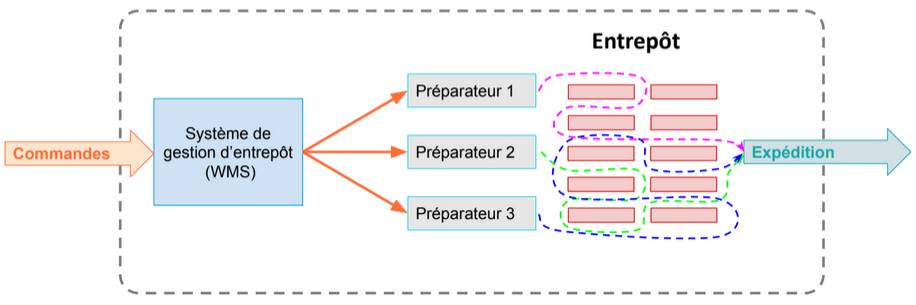
\includegraphics[width=\textwidth]{images/gestion_commandes.png}
    \caption{Traitement des commandes en entrepôt}
    \label{fig:wms_commandes}
\end{figure}

Dans le but d’augmenter l’efficacité de ces processus, les entrepôts cherchent des moyens de réduire le temps total mis par les préparateurs pour traiter les commandes. Étant donné qu’il est difficile d’agir directement sur la vitesse de déplacement d’un préparateur ou sur le temps qu’il met à manipuler un produit, l’optimisation se concentre essentiellement sur la réduction des distances parcourues dans l’entrepôt. On identifie ainsi trois axes d’amélioration permettant d’optimiser ces distances :
\begin{thematique}
\begin{enumerate}
    \item \textbf{Optimiser le \textit{picking}} : déterminer un ordre de collecte réduisant les déplacements.
    \item \textbf{Optimiser le \textit{batching}} : décider quelles commandes traiter simultanément.
    \item \textbf{Optimiser le \textit{slotting}} : organiser les produits dans l’entrepôt de manière à faciliter les collectes.
\end{enumerate}
\end{thematique}
C’est sur ces axes que Find \& Order intervient afin d’améliorer la rentabilité opérationnelle des entrepôts. L’entreprise édite une solution d’optimisation de flux destinée aux grands distributeurs et aux opérateurs logistiques, confrontés à une croissance importante du e-commerce ces dernières années. La solution est déployée en France et à l’international auprès de grands acteurs du secteur tels que Carrefour, Auchan, Bolloré Logistics ou Brico Dépôt.

\vspace{0.5cm}

Dans ce projet, nous nous concentrerons exclusivement sur le troisième axe : l’optimisation du \textit{slotting}. Il s’agit de déterminer comment organiser l’ensemble des produits dans les allées de l’entrepôt afin de réduire les distances parcourues lors des préparations. Le problème consiste donc à choisir, pour chaque produit, une position adaptée dans l’entrepôt tout en respectant les contraintes associées.

\vspace{0.5cm}

Une organisation pertinente des emplacements peut rapprocher les produits fréquemment commandés ensemble, améliorer la cohérence du cheminement dans les allées et réduire significativement la distance de déplacement. L’objectif final du \textit{slotting} est ainsi de proposer une configuration d’entrepôt plus efficace, diminuant les distances parcourues par les préparateurs et améliorant la performance globale du processus de picking et/ou batching.
\begin{thematique}
\textbf{Note sur l’usage du document}\\[3pt]
Ce document a été rédigé dans un cadre strictement pédagogique, en collaboration avec l’Université de Bordeaux.
Il contient des éléments issus de travaux internes réalisés chez Find \& Order et ne doit pas être diffusé publiquement.
Toute reproduction ou réutilisation en dehors de ce contexte pédagogique doit faire l’objet d’une demande auprès de Find \& Order.
\end{thematique}


\newpage
\section{Définitions et vocabulaire}
Avant d’aborder les objectifs du projet, il est utile de préciser quelques notions essentielles liées à l’organisation d’un entrepôt.

Un \textbf{rack} correspond à une étagère de stockage individuelle. Chaque rack dispose d’une capacité maximale, exprimée en nombre de produits, et constitue l’unité élémentaire dans laquelle les produits doivent être affectés.  
Chaque produit appartient par ailleurs à un \textbf{circuit logistique}, c’est-à-dire une catégorie regroupant des produits de même nature ou soumis aux mêmes contraintes opérationnelles.
\begin{figure}[h!]
    \centering
    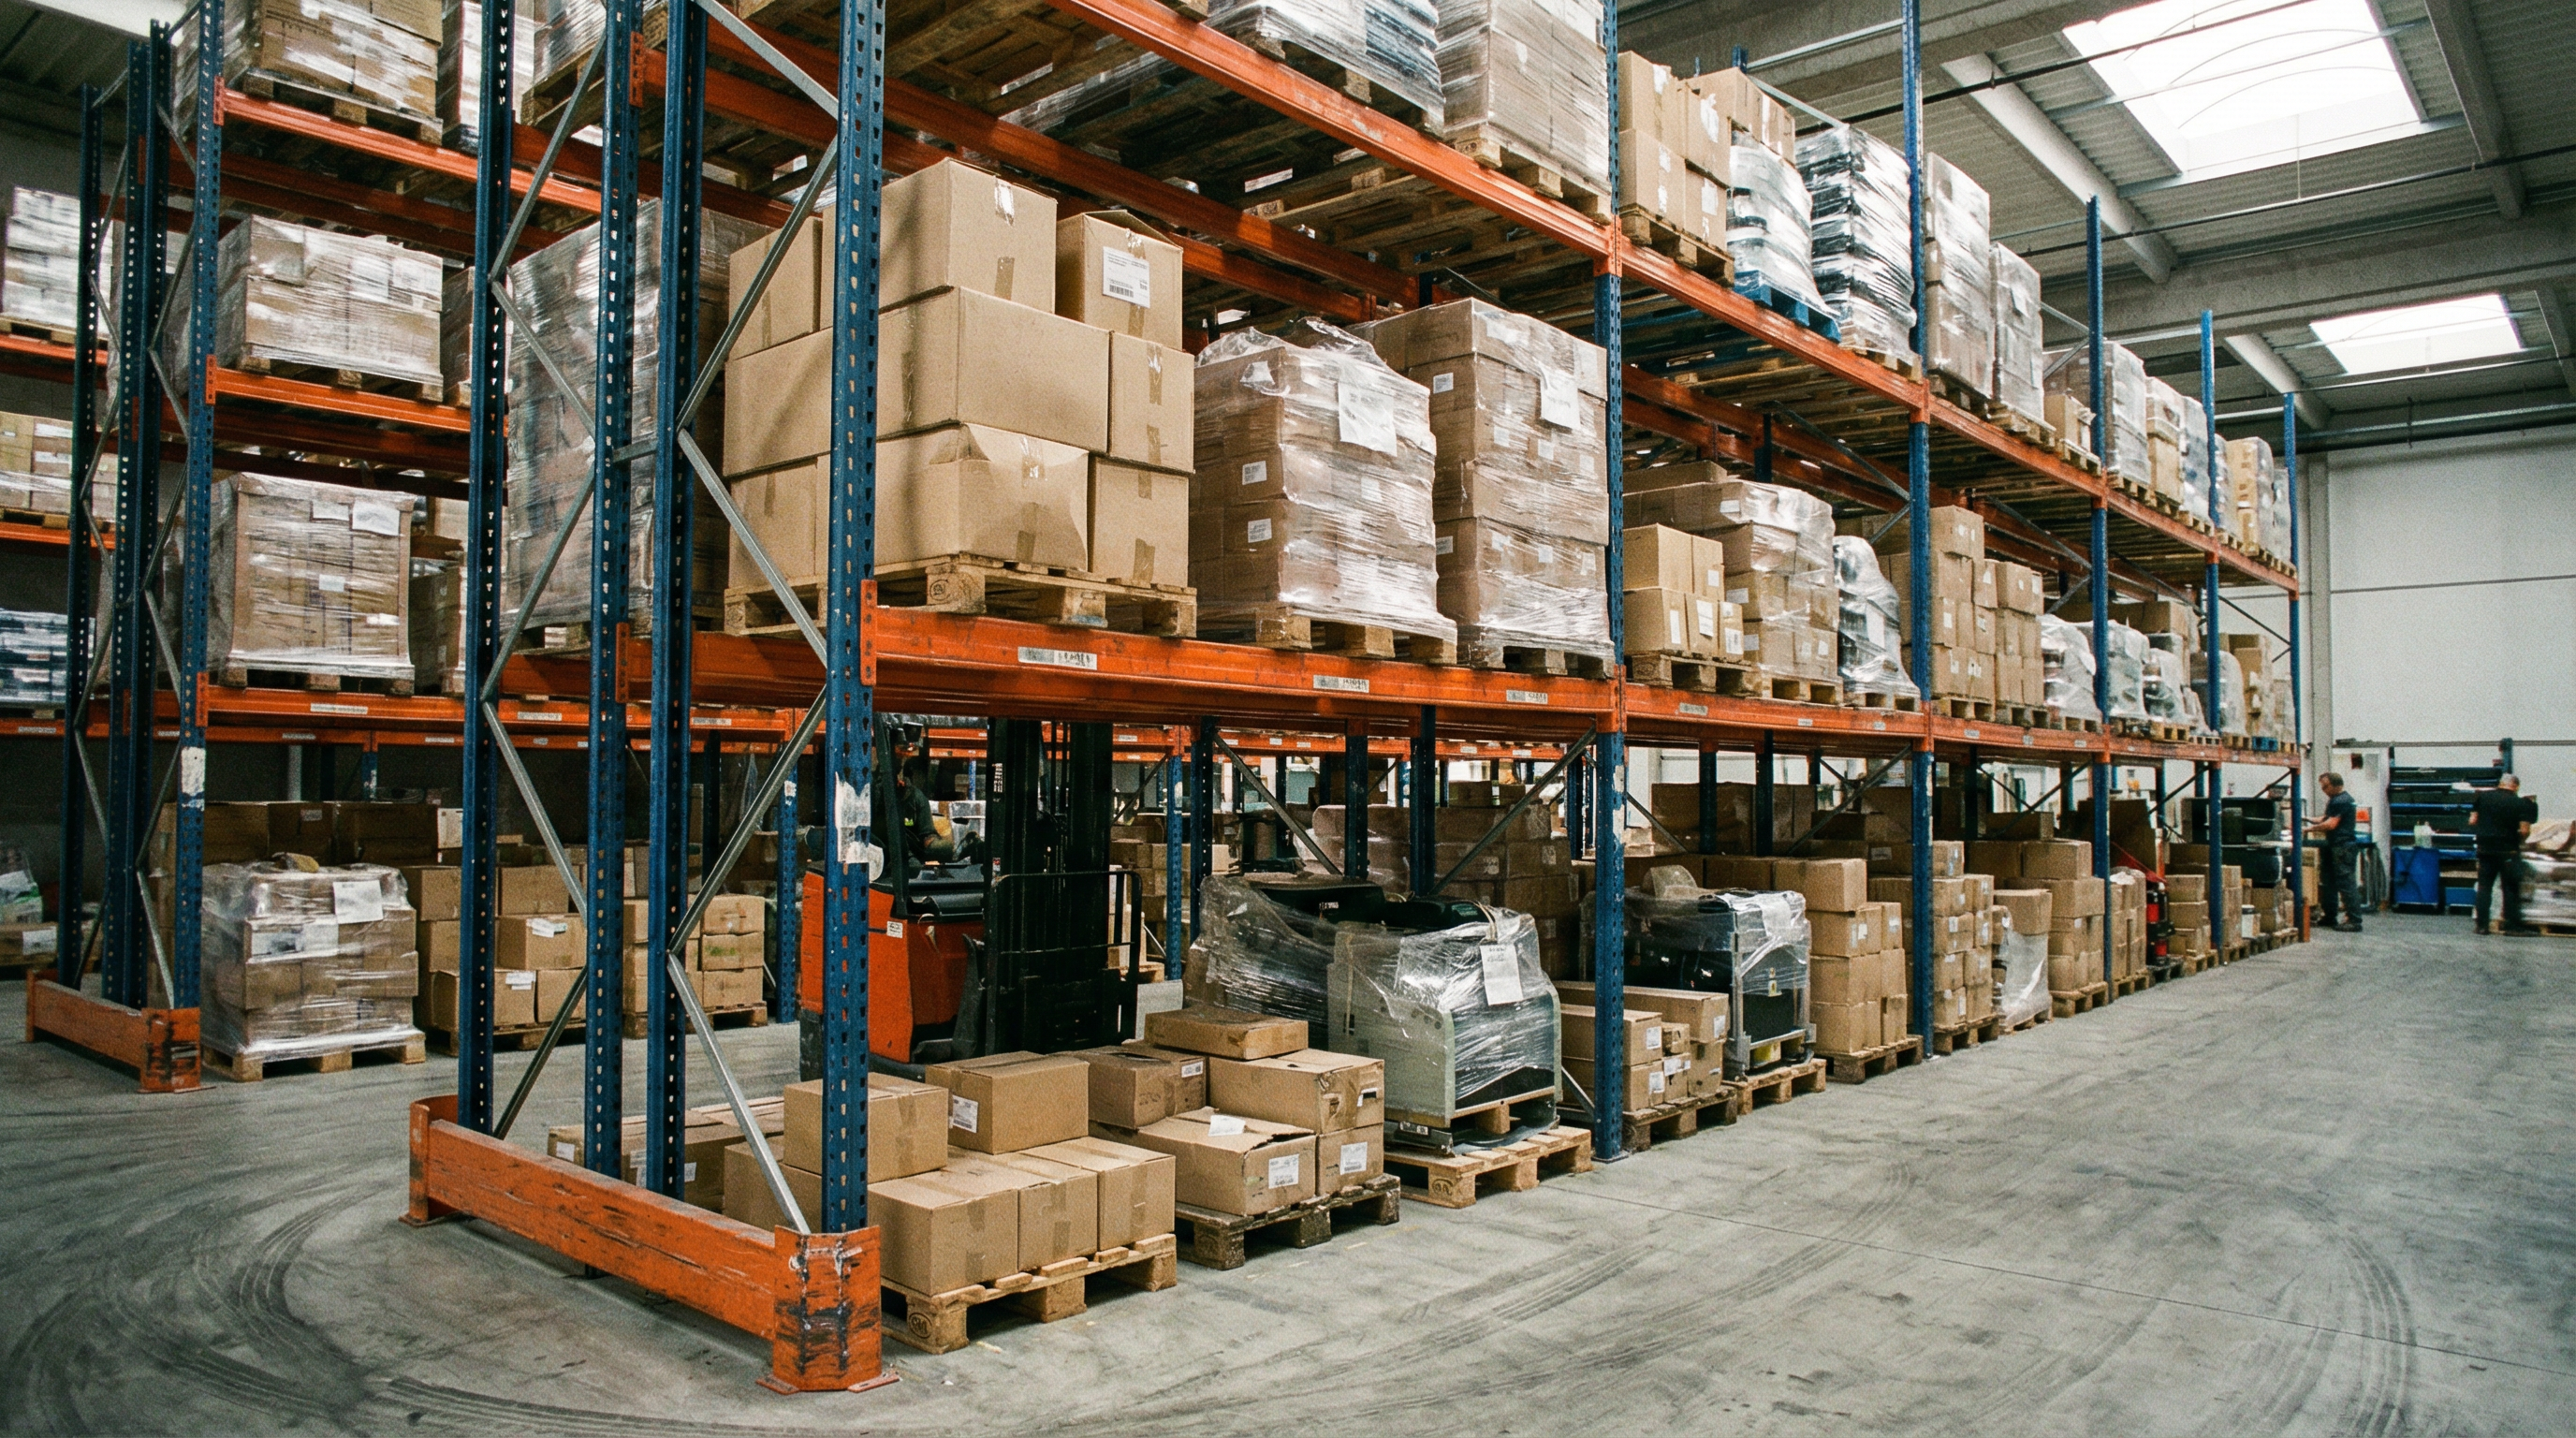
\includegraphics[width=0.45\textwidth]{images/racks.png}
    \caption{Exemple de racks dans un entrepôt logistique}
    \label{fig:racks}
\end{figure}

\vspace{0.3cm}

L'\textbf{aération} désigne les emplacements volontairement laissés vides dans les racks. Ces espaces libres sont nécessaires pour permettre la circulation, faciliter les opérations de réapprovisionnement et garantir la sécurité dans les allées.
\vspace{0.3cm}

Le fonctionnement d’un entrepôt repose également sur le \textbf{sens de circulation des allées}. Dans la grande majorité des sites industriels, une allée se parcourt dans un seul sens : le préparateur entre par une extrémité, se déplace jusqu’au bout, puis ressort de l’autre côté.  
Lorsqu’il passe à l’allée suivante, le sens de circulation s’inverse, ce qui crée un cheminement global en “S”.

Cette contrainte opérationnelle structure ce que l’on appelle un \textbf{S-PATH}.  
Elle implique qu’il n’est pas possible de visiter les racks dans un ordre arbitraire, ni de revenir en arrière dans une même allée. 
La numérotation des racks, combinée à la matrice d’adjacence fournie dans les données, permet de reconstruire automatiquement ce parcours conforme au S-PATH.  
C’est ce cheminement réel qui sera utilisé pour évaluer les distances de collecte.

\vspace{0.4cm}

Pour illustrer ce mécanisme, les deux schémas ci-dessous présentent deux cheminements valides permettant de passer d’un rack à un autre dans le respect du S-PATH :

\begin{figure}[h!]
\centering
\begin{minipage}{0.48\textwidth}
    \centering
    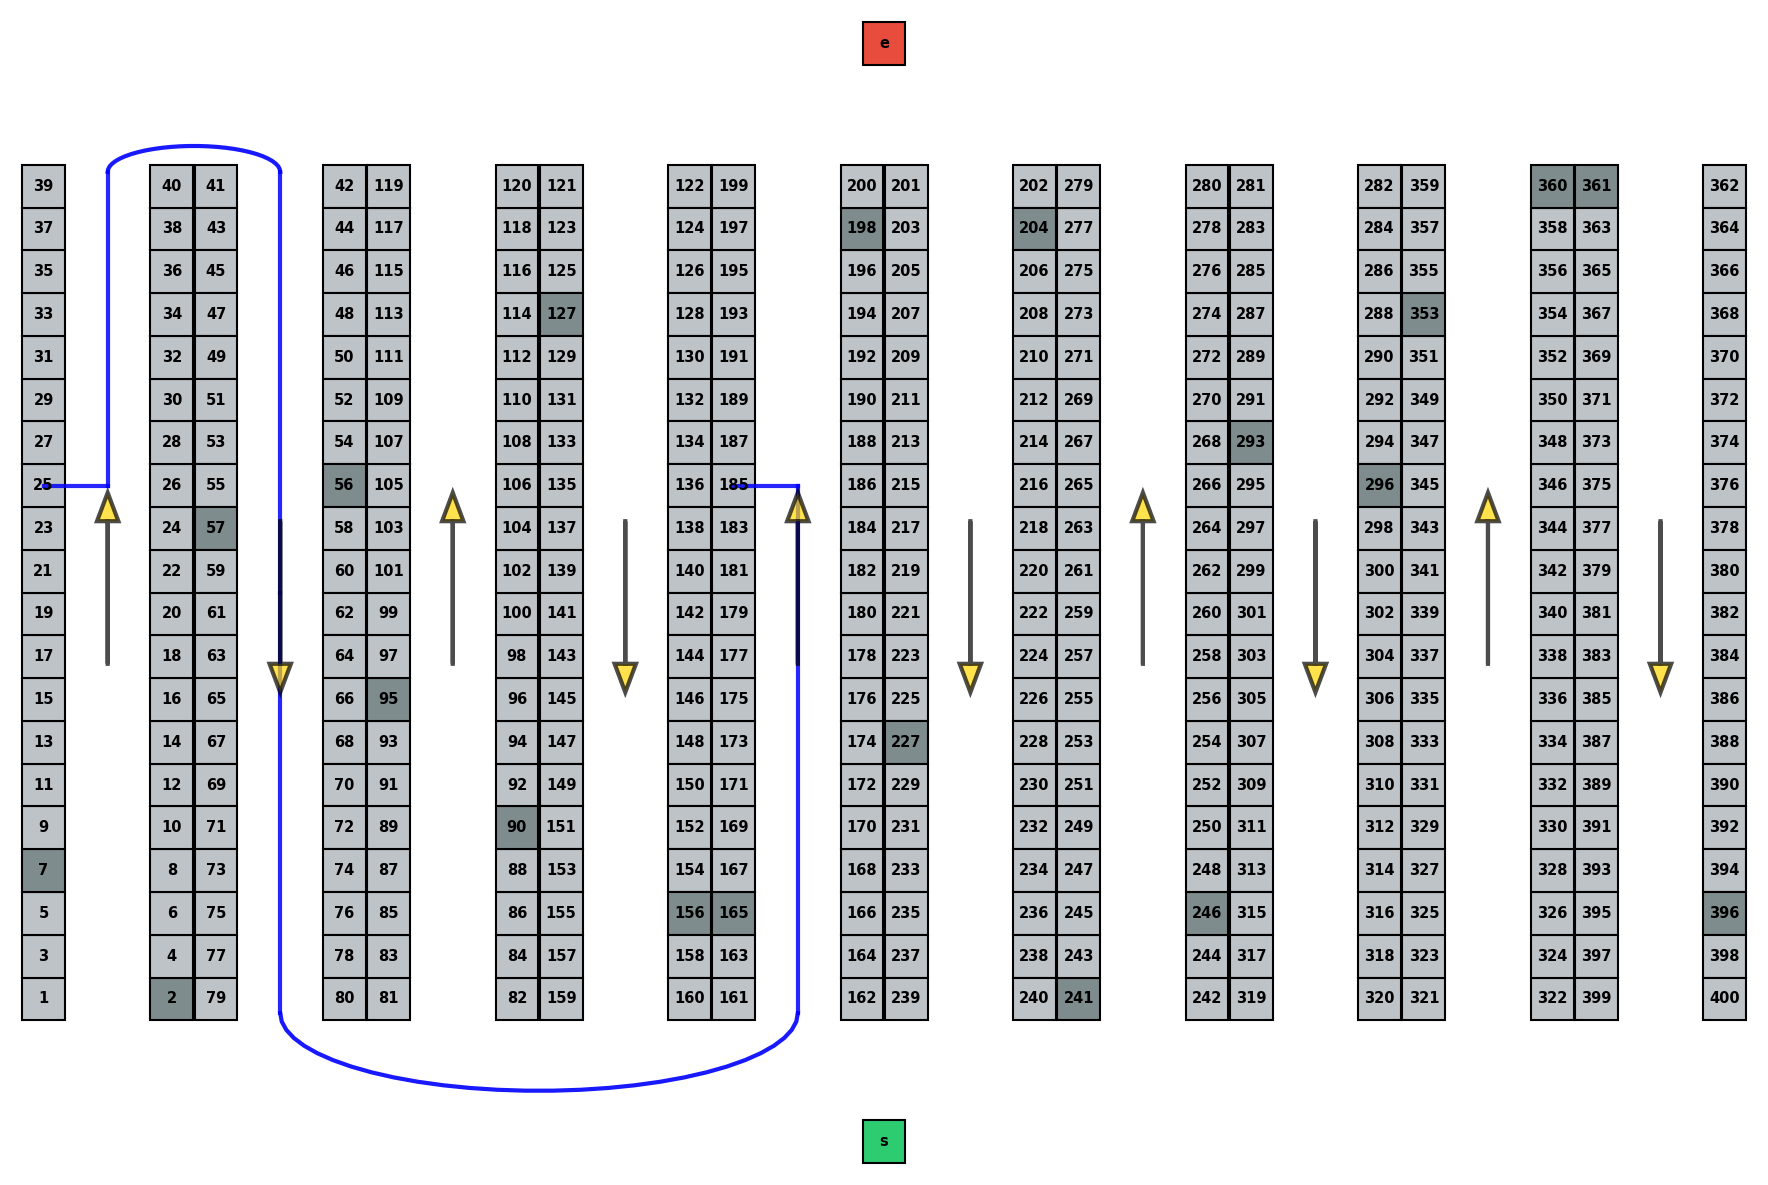
\includegraphics[width=\textwidth]{images/s_path_25_185_path_1.png}
    \caption{Cheminement n°1}
\end{minipage}
\hfill
\begin{minipage}{0.48\textwidth}
    \centering
    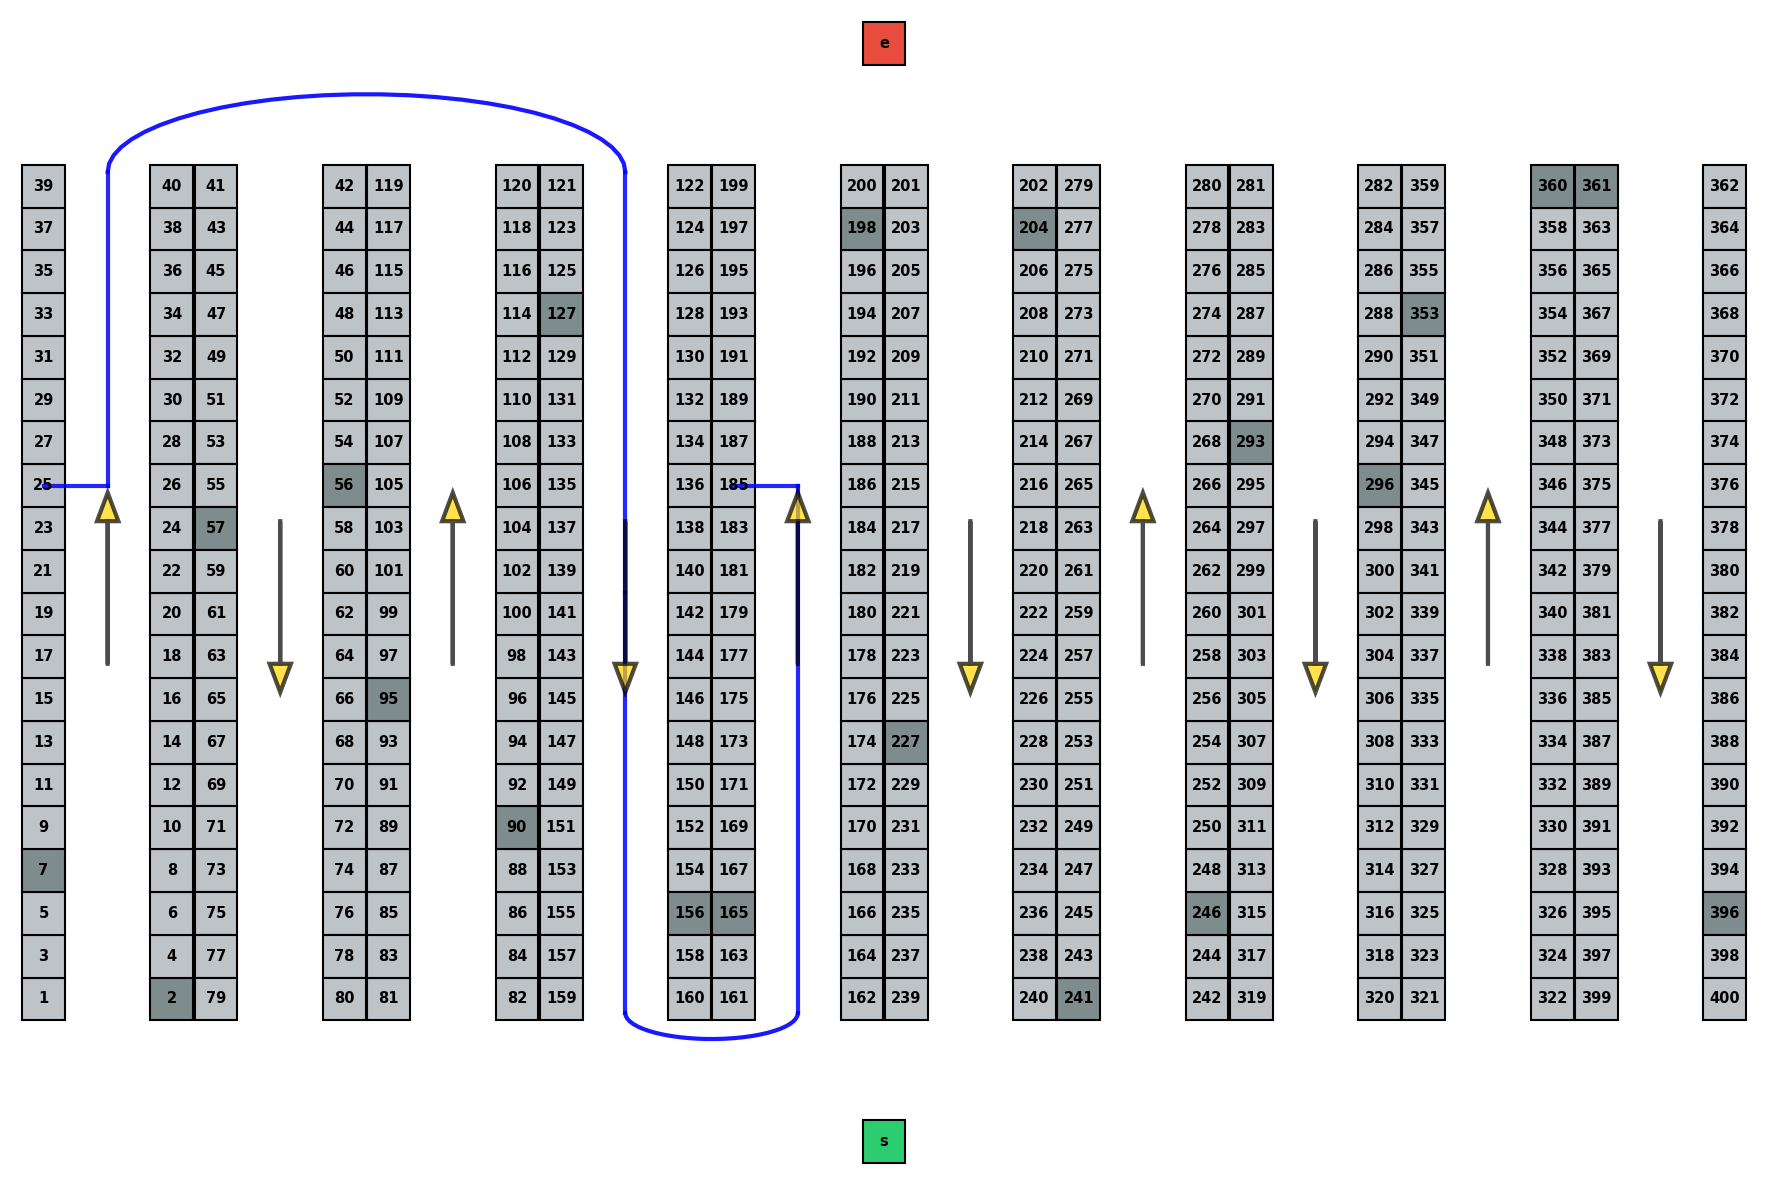
\includegraphics[width=\textwidth]{images/s_path_25_185_path_2.png}
    \caption{Cheminement n°2}
\end{minipage}
\caption{Exemples de parcours S-PATH valides pour aller du rack n\textsuperscript{o} 25 au rack n\textsuperscript{o} 185.}
\label{fig:s_path_exemples}
\end{figure}

Il est important de noter que \textbf{vous n’avez pas besoin de modéliser vous-mêmes le S-PATH}.  
Celui-ci est déjà intégré dans les distances fournies : par exemple, sur la figure \ref{fig:s_path_exemples} la distance entre le rack 26et le rack 185 correspond directement au plus court S-PATH permettant de passer d'un rack à l'autre. Pour collecter les produits d’une commande, le cheminement respectant le S-PATH consiste à \textbf{visiter les racks dans l’ordre croissant de leur numérotation}, cet ordre correspondant exactement au parcours réel imposé par le sens de circulation des allées.
\newpage
\section{Attendu du projet}

Dans ce projet, vous disposerez d’une description complète d’un entrepôt : sa structure physique, l’ensemble de ses racks, les distances entre eux, leurs capacités de stockage, ainsi que la liste des produits et des commandes. À partir de ces données, votre objectif sera de proposer une nouvelle organisation des produits dans l’entrepôt, en respectant les contraintes de capacité et en cherchant à réduire les distances de collecte. 

Une solution valide consiste donc à affecter chaque produit à un rack en respectant ces capacités, tout en construisant une organisation cohérente et efficace.


\vspace{0.4cm}

Les fichiers fournis décrivent l’ensemble des informations nécessaires :

\begin{itemize}
    \item Les \textbf{capacités des racks}, précisant pour chacun le nombre maximal de produits qu'il peut contenir. Cela inclut certains racks particuliers de capacité 0 représentant par exemple le point de départ et le point d'arrivée.
    \item Une \textbf{matrice d'adjacence} indiquant les distances entre tous les racks de l'entrepôt.
    \item Le \textbf{circuit} associé à chaque produit, correspondant à sa catégorie logistique.
    \item La \textbf{décomposition en allées}, listant les racks présents dans chaque allée.
    \item L'ensemble des \textbf{commandes}, correspondant au carnet de commandes du problème.
    \item Le \textbf{taux d'aération minimal} à respecter dans chaque allée.
\end{itemize}
\vspace{0.4cm}


À partir de ces données, vous devrez construire une solution de \textit{slotting} : une affectation complète de tous les produits vers les racks, satisfaisant les contraintes de stockage, tout en garantissant une organisation cohérente avec les circuits logistiques auxquels appartiennent les produits. L’objectif est de proposer une configuration respectant ces contraintes et minimisant le coût total défini dans la section Évaluation.


\vspace{0.2cm}

Afin de faciliter votre prise en main du sujet, une petite instance d'exemple (« instance jouet ») ainsi qu'un \textit{checker} vous seront fournis.  Une instance taille réelle vous sera également fournie. Les formats détaillés des fichiers sont décrits dans le document \texttt{SPECIFICATION\_FORMATS.md}.


\section{Contraintes du slotting}

Pour organiser efficacement l’entrepôt, vous devrez décider comment répartir les différents circuits logistiques au sein des allées. La configuration finale doit respecter plusieurs contraintes structurelles essentielles afin de garantir un fonctionnement réaliste et cohérent.

\paragraph{Aération.}
Un pourcentage \textbf{minimum} de la capacité de chaque allée doit être réservé à l'aération. Ces emplacements vides représentent les marges nécessaires à la circulation, à la sécurité et aux contraintes opérationnelles. Le taux d'aération fourni constitue un \textbf{plancher} : chaque allée doit conserver au moins ce pourcentage d'emplacements libres.

Si le nombre total de produits à placer est inférieur à la capacité totale moins l'aération minimale, vous disposerez naturellement d'emplacements vides supplémentaires. Vous êtes libre de répartir cette aération excédentaire comme vous le souhaitez dans l'entrepôt.
\paragraph{Capacité des racks.}
Chaque rack possède une capacité maximale exprimée en nombre de produits qu’il peut accueillir.  
L’affectation finale doit respecter ces limites : il est interdit de dépasser la capacité d’un rack.
\paragraph{Contiguïté.}
Les produits d'un même circuit doivent être regroupés dans un intervalle continu de racks.
Plus précisément, si l'on note $[r_{\min}, r_{\max}]$ l'intervalle des racks contenant les produits d'un circuit, alors les intervalles de deux circuits distincts ne peuvent pas se chevaucher (sauf éventuellement en un seul rack frontière commun comme illustré sur le rack n°15 de la figure \ref{fig:config_1}).

Il est tout à fait possible que des racks vides (aération) ou des racks de capacité nulle (obstacles, points de passage) se trouvent à l'intérieur de l'intervalle d'un circuit : cela ne viole pas la contrainte de contiguïté.


\vspace{0.1cm}

\paragraph{Exemple illustratif.}  
Étant donnée une configuration d’aération fixée arbitrairement, les deux figures ci-dessous présentent deux répartitions possibles des 4 circuits dans l’entrepôt.  

Sur la Figure~\ref{fig:config_1}, les circuits sont organisés selon la permutation $(3,1,4,2)$, tandis que la Figure~\ref{fig:config_2} montre la permutation $(1,2,3,4)$.  

Les flèches visibles au centre des allées représentent le sens de circulation selon le \textit{S-path} : une fois engagé dans une allée, l’opérateur la parcourt intégralement sans revenir en arrière.

\begin{figure}[h!]
\centering
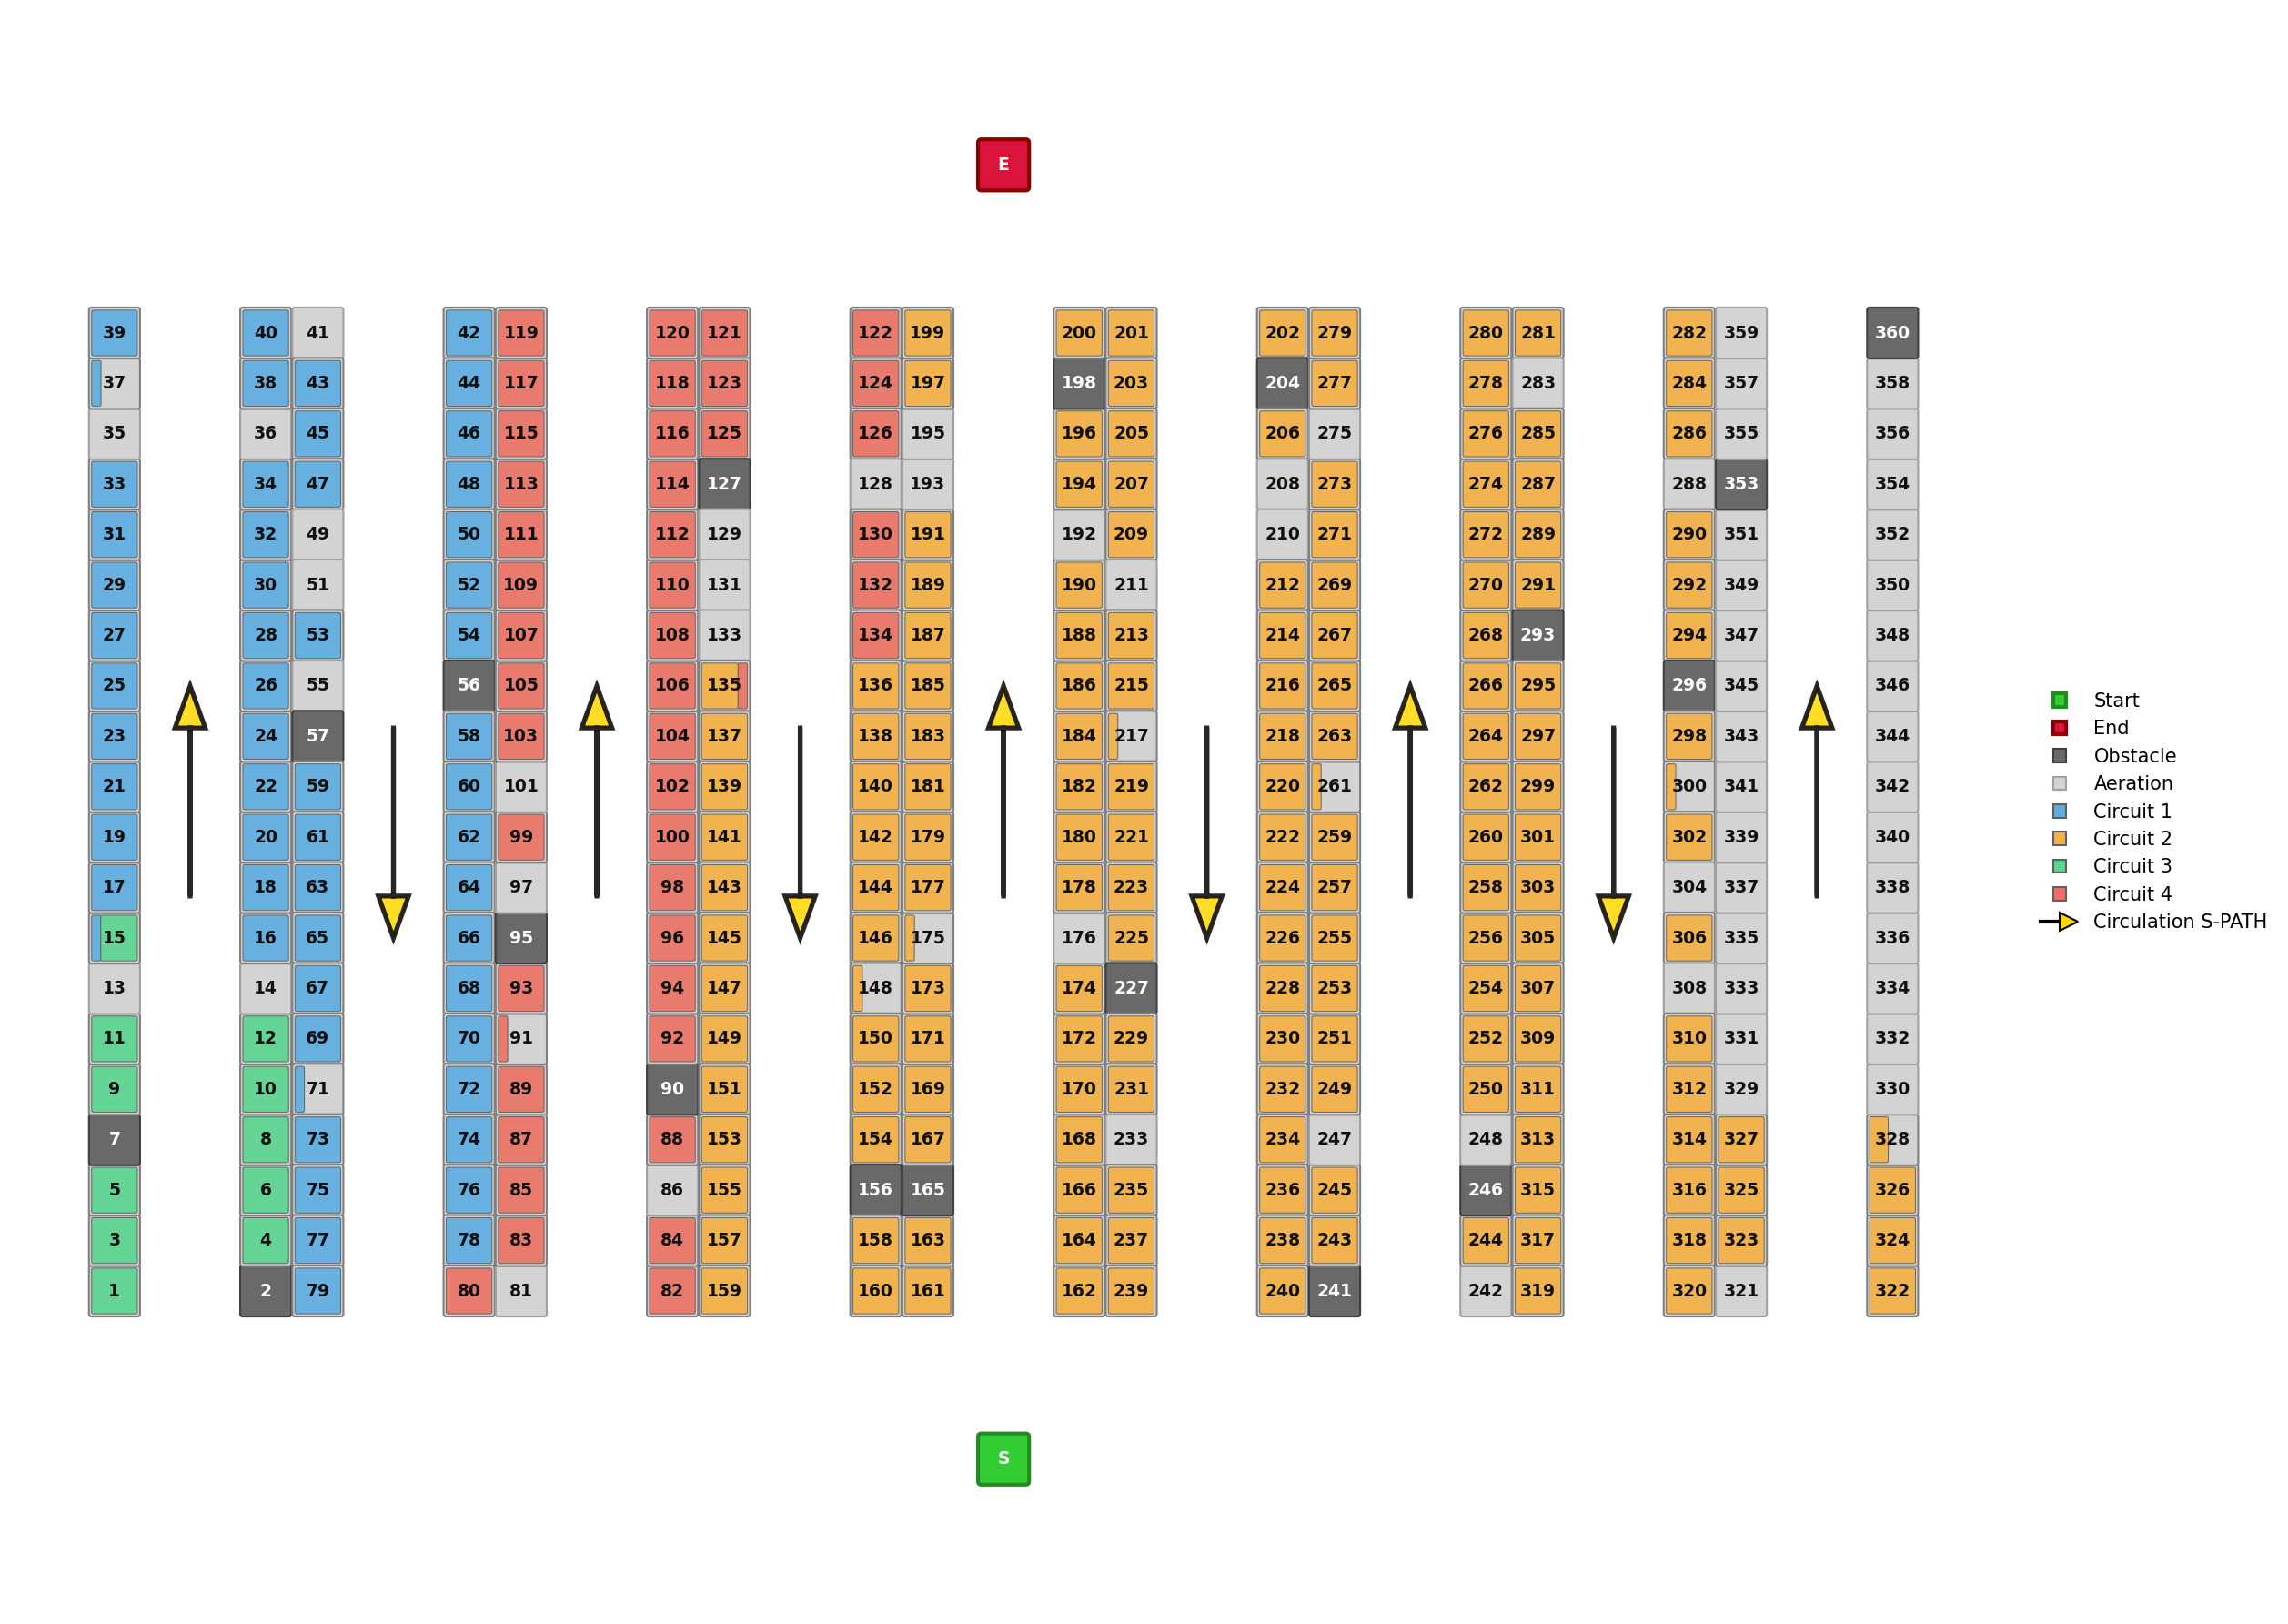
\includegraphics[width=0.95\textwidth]{images/warehouse_plot_v2.png}
\caption{Configuration correspondant à la permutation $(3,1,4,2)$}
\label{fig:config_1}
\end{figure}

\begin{figure}[h!]
\centering
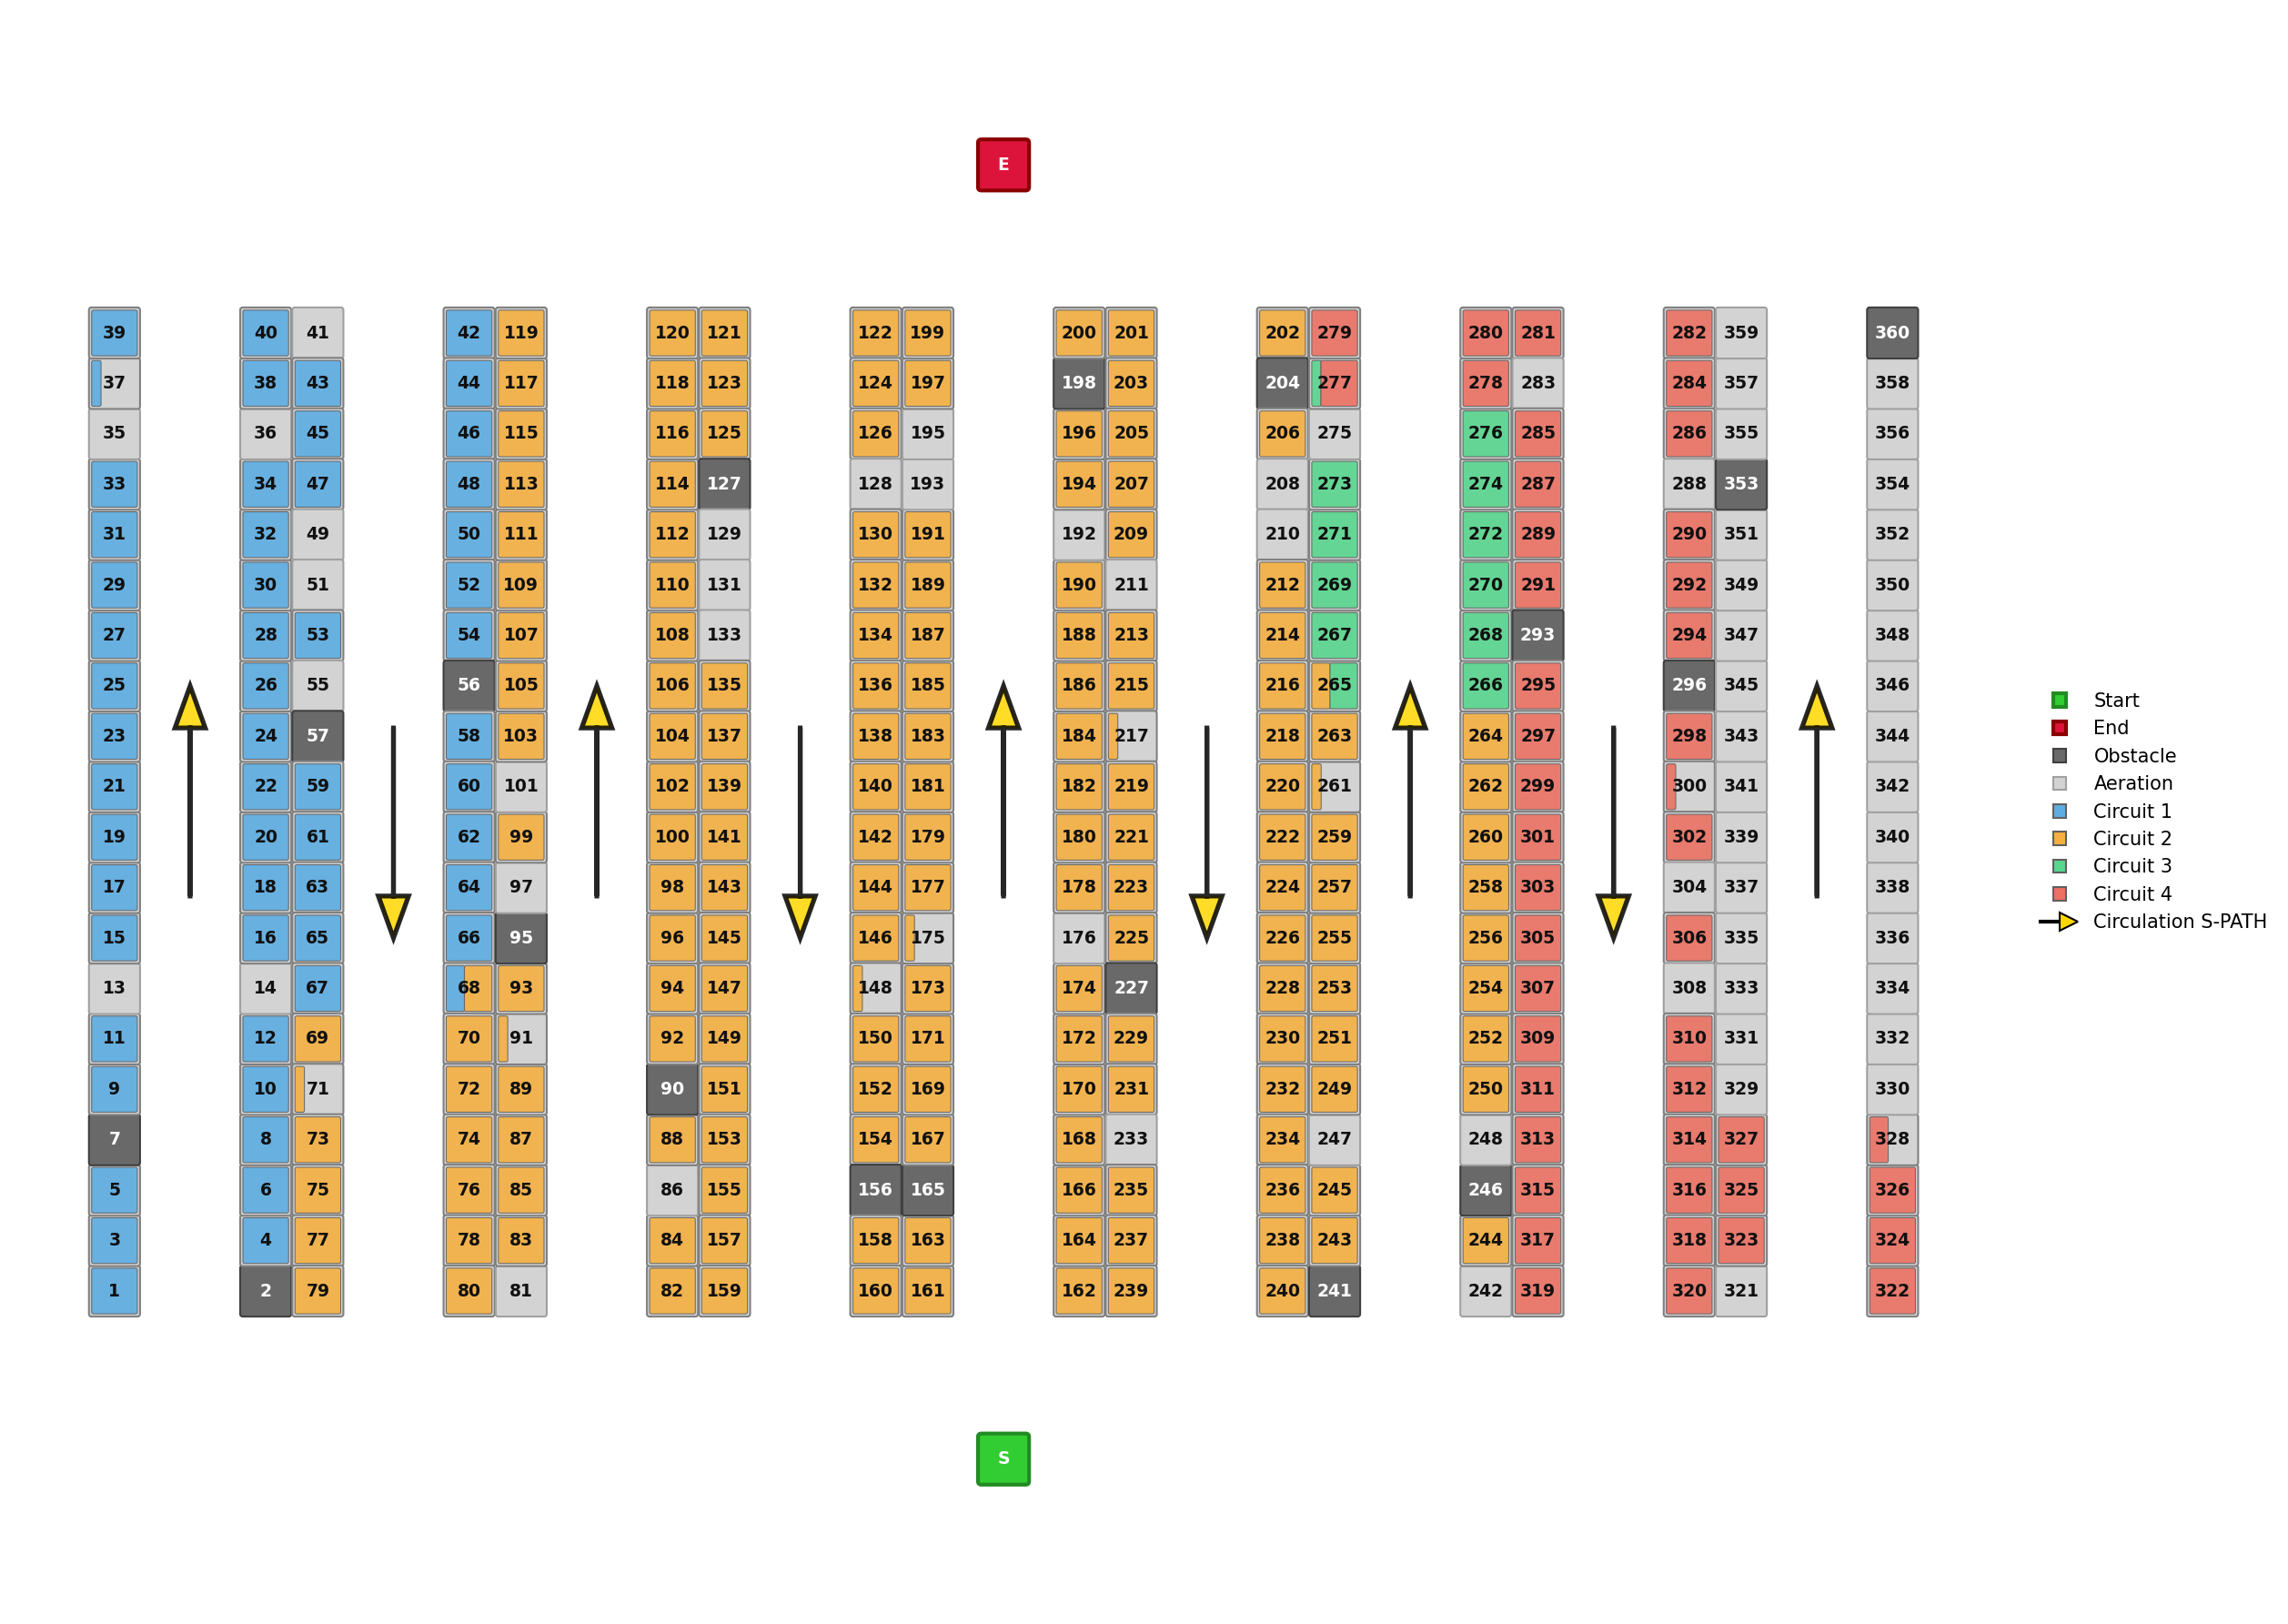
\includegraphics[width=0.95\textwidth]{images/warehouse_plot.png}
\caption{Configuration correspondant à la permutation $(1,2,3,4)$}
\label{fig:config_2}
\end{figure}

\newpage
\section{Évaluation}

Une fois votre solution de \textit{slotting} construite, elle doit être évaluée à partir des distances réellement parcourues pour préparer les commandes.  
Chaque commande est constituée d’une liste de produits : l’organisation finale des racks influe donc directement sur les déplacements nécessaires pour aller les collecter.

\subsection{Coût d’une commande}

Le calcul du coût repose sur le cheminement réel imposé par l’entrepôt.  
Les allées possèdent un sens de circulation fixé (le \textit{S-path}), ce qui détermine l’ordre dans lequel les racks peuvent être visités.  
Dans ce cadre, la collecte des produits d’une commande s’effectue en visitant les racks concernés dans l’ordre croissant de leur numérotation.

Le parcours complet est donc défini comme suit :
\begin{enumerate}
    \item partir du rack représentant le point de départ ;
    \item visiter les racks contenant les produits de la commande, dans l’ordre croissant de leur numérotation ;
    \item rejoindre le rack représentant le point d’arrivée.
\end{enumerate}

Les points de départ et d'arrivée sont eux-mêmes modélisés comme des racks de capacité nulle. Par convention, le \textbf{rack 0} représente le point de départ et le \textbf{rack $n-1$} (dernier rack) représente le point d'arrivée.

\subsection{Coût total d’une solution}

Le coût global d’une solution de \textit{slotting} est obtenu en agrégeant le coût de toutes les commandes :

\[
\text{solutionCost} = \sum_{\text{commandes}} cost(\text{commande})
\]

Une solution est d’autant plus efficace que ce coût global est faible.


\subsection{Exemple illustratif}

Considérons l’exemple représenté sur la Figure~\ref{fig:exemple_s_path}.  
Dans cet exemple, les produits de la commande sont répartis dans les racks suivants :

\[
[26,\ 74,\ 140,\ 260]
\]

Supposons que la commande contienne 10 produits organisés comme suit :

\begin{center}
\begin{tabular}{|c|cccccccccc|}
\hline
\textbf{Produit} & a & i & h & b & c & e & f & g & d & j \\
\hline
\textbf{Rack}    & 26& 26& 26& 74 & 74 & 74 & 74 & 74 & 140 & 260 \\
\hline
\end{tabular}
\end{center}


Même si plusieurs produits sont stockés dans un même rack, chaque rack n’est visité qu’une seule fois.  
Le cheminement réel imposé par le \textit{S-path} consiste donc à :

\begin{enumerate}
    \item partir du rack \textbf{s} (point de départ) ;
    \item visiter successivement les racks par étiquetage croissant \textbf{26→ 74 → 140 → 260} ;
    \item rejoindre le rack \textbf{e} (point d’arrivée).
\end{enumerate}

Le coût de cette commande correspond alors à: 

\[
\text{cost} =
D(s,26)
+ D(26,74)
+ D(74,140)
+ D(140,260)
+ D(260,e)
\]

où chaque terme \(D(i,j)\) est directement la valeur indiquée dans la matrice d’adjacence, laquelle encode déjà la plus courte distance réalisable entre les racks $i$ et $j$ en respectant le S-path. Cet exemple montre qu’une commande comportant de nombreux produits peut n’entraîner que la visite d’un petit nombre de racks.

\begin{figure}[h!]
\centering
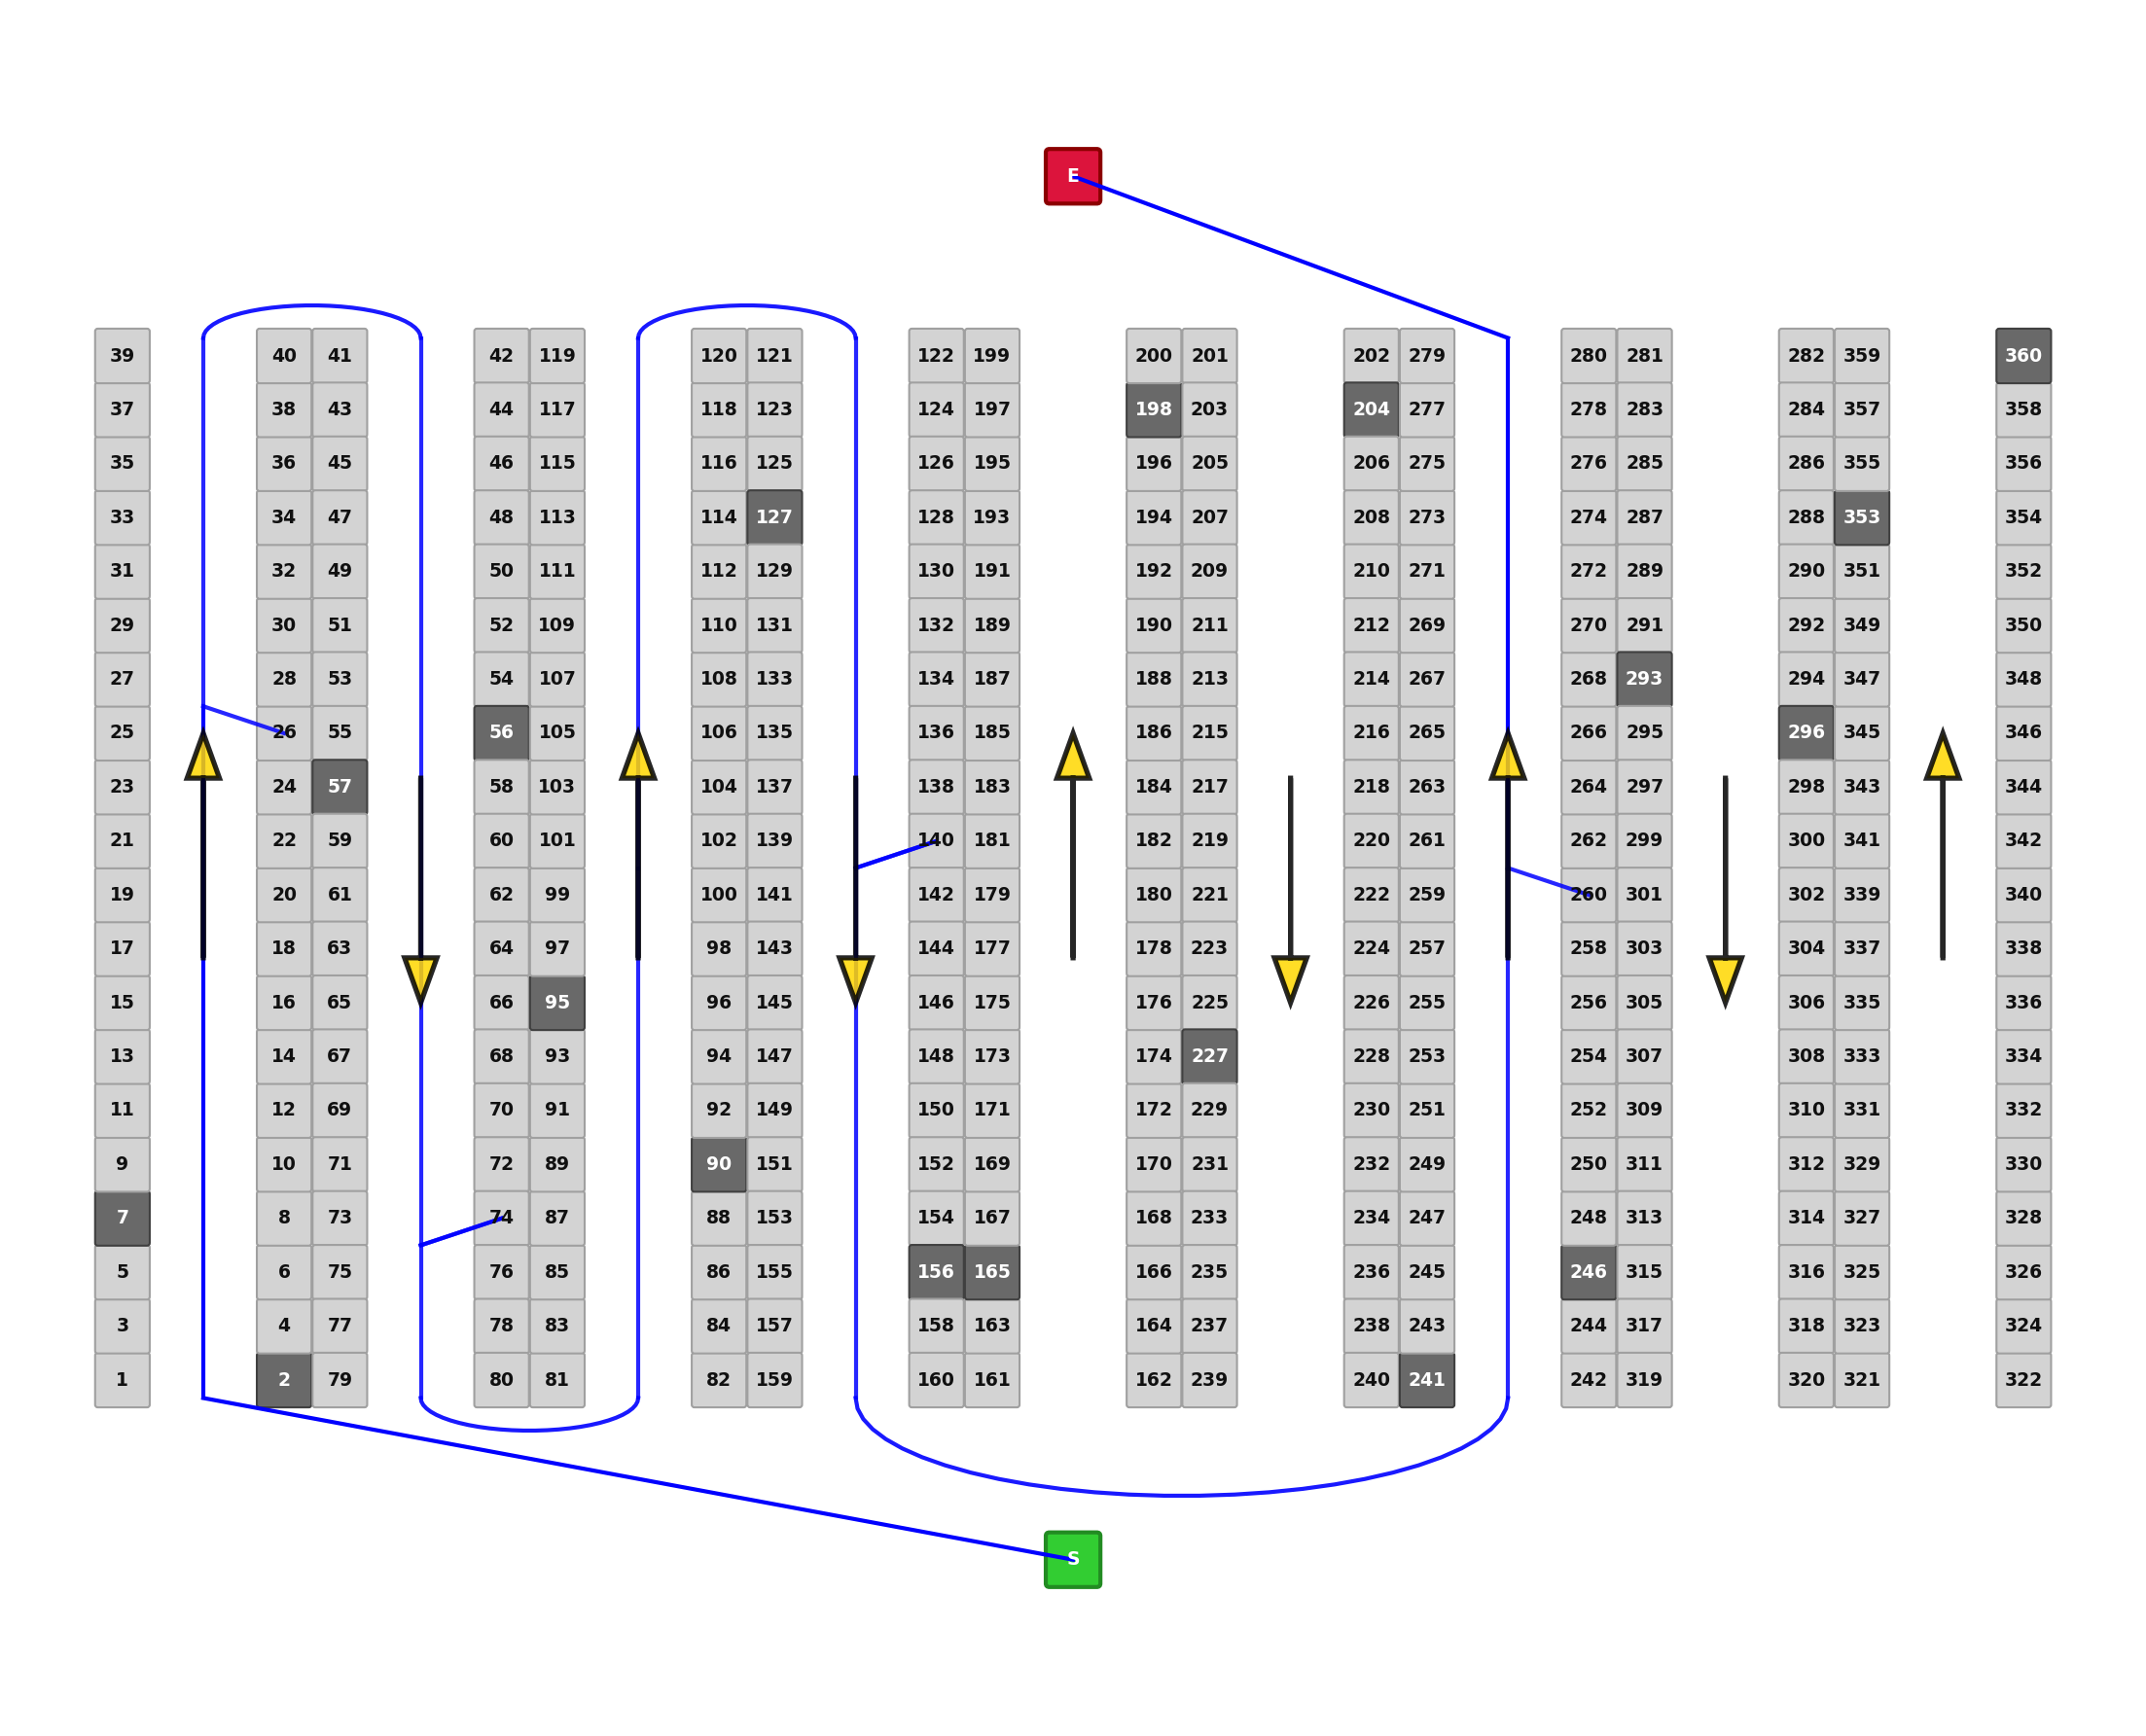
\includegraphics[width=\textwidth]{images/s_path_26_74_140_260_v3.png}
\caption{Exemple de parcours S-PATH pour une commande visitant les racks 26, 74, 140 et 260.}
\label{fig:exemple_s_path}
\end{figure}





\end{document}

% Document et projet réalisé par Valentin Guidon
